\section{Discussion}\label{discussion}

\subsection{Time evolution}\label{discussion:normal}

We have seen in Sect.~\ref{results} that density-weighted VSFs reflect a combination of uniform, compressible turbulence, large-scale shocks, and gravitational collapse.  Extended self-similarity emphasises the turbulent nature of these high-Reynolds numbers flows even in regions of gravitational collapse. 

The impact of SN shocks hitting the clouds is to inject power at all scales (Fig.~\ref{pic:results:vsf_example}). 
The resulting VSFs tend to lose their power-law character. Fitting a power-law to them anyway results in substantial perturbations from the predictions for compressible turbulence even under extended self-similarity.
Fig.~\ref{pic:results:z_all} shows times of SN explosions and periods of strong accretion onto the clouds. 
\textbf{Remembering that it can take the shock front more than 1~Myr to propagate from the site of the SN explosion to the molecular cloud,} perturbations in $Z$ not associated with zero-crossings by $\zeta(3)$ are consistent with being caused by SN shock front interactions with the clouds.  
These shock interactions last for only a fraction of a megayear, though, 
\textbf{consistent with the crossing time of the blast wave through the dense interior of the cloud}, after which the turbulent nature of the flow reasserts itself.

As the clouds gravitationally collapse, the resulting increase in small-scale power flattens or even inverts the density-weighted VSFs, resulting in decreasing or even negative values of $\zeta$ (Fig.~\ref{pic:results:zeta_all}(a)). The increase in small-scale power can also be derived from the increasingly negative binding energy of the clouds as further gas falls into them \citepalias{IbanezMejia2017}. 
\textbf{
At the same time as the turbulence becomes increasingly non-uniform and anisotropic because of the importance of gravitation, the bulk velocity dispersion of the cloud increases.
\citetalias{IbanezMejia2016} showed that Eq.~(\ref{eq:larson}) is satisfied at these late times, but not at early times, less than a free-fall time, when the velocity dispersion inherited from the background turbulent flow is independent of the size of the cloud. 
These early times are when the turbulence dominates the flow and the second-order power law is roughly $\zeta(2) \simeq 1/2$.
This suggests that the apparent agreement with Larson's size-velocity relationship is coincidental, but also that observing two-point correlations using a method that cannot capture the dense flows adequately will yield this result, thus perhaps explaining the apparent success of such efforts.
}

Extended self-similarity shows VSF ratios characteristic of compressible turbulence (Fig.~\ref{pic:results:z_all}a), as can be seen from their tending to lie between the incompressible limit of \citet{She1994} and the extremely compressible Burgers turbulence limit of \citet{Boldyrev2002}.
(The extended self-similarity procedure fails as $\zeta(3)$ passes through zero, however, so it must be interpreted in concert with the raw values of $\zeta$.)
\textbf{This suggests that, just as the extended self-similarity procedure removes the effects of dissipation, it also removes the effects of hierarchical gravitational collapse, while continuing to reflect the turbulence in these high Reynolds-numbers flows.}


\subsection{Line-of-sight velocities}\label{discussion:1d}

In Sect.~\ref{results:1d} we have seen that the $\zeta$ and $Z$ derived from the 1D VSFs generally evolve similarly to those derived from the 3D VSFs.
Yet, we have also seen that individual sight lines may evolve differently.
These differences appear to reflect the detailed geometry of shock impacts on the cloud, which are reflected more strongly in the higher-order VSFs.
For example, for the first 2~Myr of the evolution of \texttt{M4} the values of $Z$ along the $y$-axis are significantly higher than those observed along the other axes and diverge significantly from the values expected for uniform turbulence.
Recall that a perturbation in $Z$ usually corresponds to an episode of strong shock driving, suggesting an impact along the $y$-axis at this time. 
Along the other two axes, $Z$ continues to agree with supersonic turbulence \citep{Boldyrev2002}.
This effect is only visible as we analyse the three dimensions separately, while the driving of the gas along the $y$-axis is averaged out in the 3D VSFs (see Fig.~\ref{pic:results:z_all}a).

In summary, for a fully developed 3D turbulent field we expect that 1D VSFs behave similarly to 3D VSFs.
However, when there is a preferred direction along which the gas flows, the 1D and 3D VSFs differ significantly from each other. 
Thus, we predict that observed VSFs reflect the nature of turbulence within MCs unless there is clear evidence that the gas is driven in a particular direction (e.g., by a stellar wind or SN shock front).

Note that this analysis does not take typical line-of-sight effects, such as optical depth or blending, into account. 
Future studies need to investigate this point in more detail by performing VSF analyses based on full radiative transfer calculations.



\subsection{Density thresholds}\label{discussion:densthres}

We find that the structure and behaviour of VSFs strongly depends on whether or not we assume a density threshold in computing them.
In the fiducial case, where n$_\mathrm{cloud}$~=~100~cm$^{-3}$, we have seen a mostly straight decline of $\zeta$ while $Z$ remains fairly constant over time, reflecting the contraction of the clouds due to self-gravity.
On the other hand, if we remove the density threshold, including the entire high-resolution \textbf{cube} in the calculation, we observe a completely different picture.
The high velocities present in the diffuse interstellar medium surrounding the cloud lead to strong large-scale power and thus much steeper VSFs, corresponding to higher values of $\zeta$. 
There is still a slightly declining trend in $\zeta$, but the evolution is dominated by random fluctuations.
We also see that $Z$ remains constant for the entire simulation in every case.
The VSFs for the entire box appear consistent with the prediction for the value in incompressible turbulence \citep{Boldyrev2002}. 
This suggests that they are dominated by the subsonic flow in the hot gas with $T > 10^6$~K that occupies most of the volume of the box.

\textbf{
Furthermore, the results demonstrate that the effect of SNe, and the interaction of the produced shock fronts with the ISM acts rather locally. 
This means that a single SN can not drive the gas dynamics on scales of our entire cubes (40$^3$~pc$^3$), at least not in the same way as it does on scales of individual MCs.
Rather the VSFs reflect the superposition of multiple SNe that only combined drive the turbulence of the diffuse ISM.
}

We conclude that the decision of whether or not a density threshold is used has a significant and direct influence on the resulting VSFs.
Indeed, it is a straight-forward approach to focus the analysis on the actual area of interest.
In observational studies such a threshold will anyway always be present as minimal collision rates for excitation or the sensitivity of detectors automatically introduce implicit density or intensity thresholds. 
Although we have only tested two specific setups in this context we have seen the significance of a proper choice of the density threshold, as well as a proper discussion of the obtained results considering the threshold as one of the defining parameters.




\subsection{Density weighting}\label{discussion:densweight}

In this subsection, we discuss the effect of computing the VSF with or without including density weighting, relying on the results presented in Sect.~\ref{results:densweight}.
As long as the turbulence is dominated by the large scales, and a density threshold is used, considering the density weighting does not have a significant effect.
However, as the clouds evolve the differences increase:
the non-weighted VSFs never drop below 0.5.
This is because the non-weighted VSF treats all cells equally, no matter whether the particular cell represents a dense element of the cloud centre or a diffuse element of the cloud's edge, while the weighted VSF gives more weight to the matter within the small-scale, dense, collapsing regions.
The kinetic energy is dominated by these regions.
Thus, neglecting density weighting decouples the VSF from the kinetic energy distribution.  \textbf{(A more exact treatment of this question is given by \citet{Kritsuk2013a} and \citet{Banerjee2017,Banerjee2018}.)}
This is particularly important at late times when small-scale collapse dominates.

Nevertheless, Fig.~\ref{pic:results:z_all}(d) illustrates that these differences do not prevent extended self-similarity from holding. 
Regardless of whether density-weighting is included, the values of $Z$ remain similar, with similar responses to external driving, except for the features created when $\zeta(3)$ passes through zero in the density-weighted VSFs.
This observation is true for all Jeans refinement levels, as Fig.~\ref{pic:results:comp_weighting} demonstrates.


\begin{figure*}
	\centering
    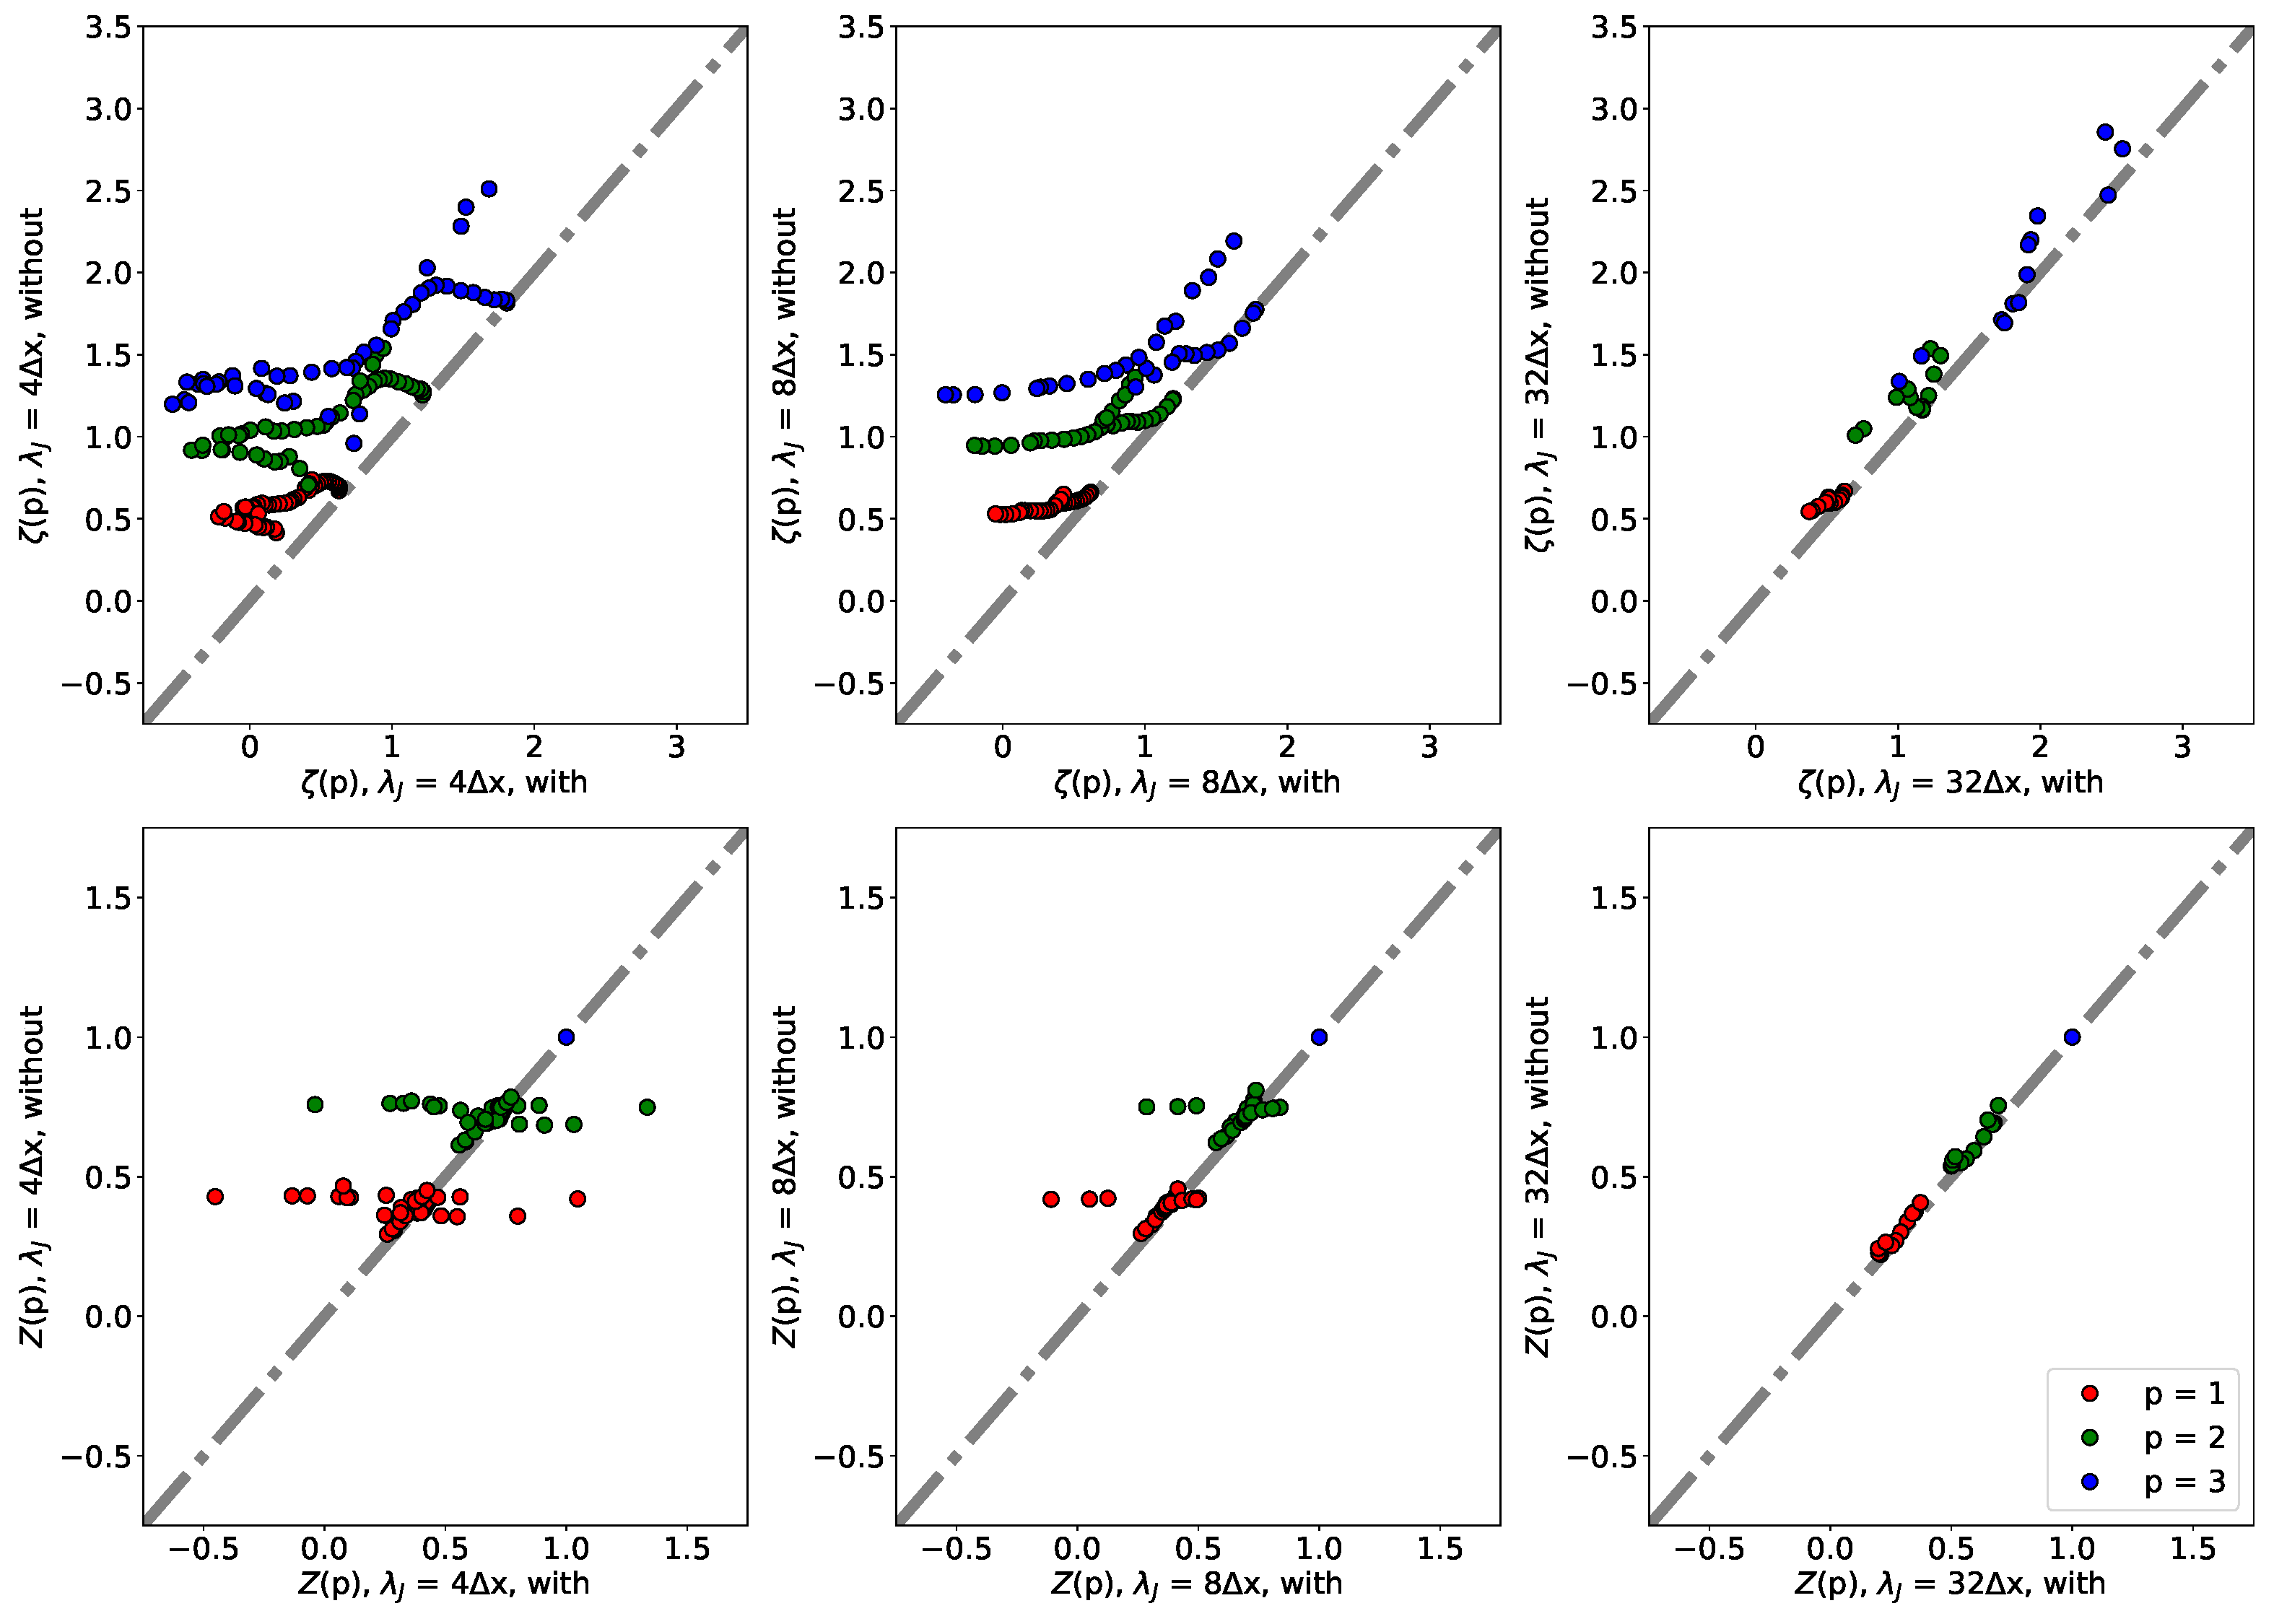
\includegraphics[width=\textwidth]{comp_weighting.pdf}
    \caption{ Comparison of $\zeta$ (\textit{top}) and $Z$ (\textit{bottom}) measured based on density-weighted VSFs (\textit{abscissas}) and non-weighted VSFs (\textit{ordinates}). We note that the given values are based on \texttt{M3} only.}
    \label{pic:results:comp_weighting}
\end{figure*}

Fig.~\ref{pic:results:comp_weighting} summarises the comparison of $\zeta$ and $Z$ measured with the density-weighted and non-weighted VSFs for all Jeans refinement levels (meaning the granularity used for modelling the turbulent motions of the gas, see Sect.~\ref{results:refinement} for more details).
The figure clearly shows that the measurements only agree well for the highest refinement level with $\lambda~=~32\Delta x$.
However, we would need more data points to be sure that this correlation is indeed real.
At lower refinement levels the measurements, as those used for the standard analysis and all other test scenarios but the one presented in Sect.~\ref{results:refinement}, correlate less well with each other. 
The differences in the samples appear dominantly when the density-weighted $\zeta$ cease below $\approx$0.5, which is the global minimum for the non-weighted $\zeta$. 
This means that none of the $\zeta$ computed in all clouds and refinement levels with the non-weighted VSF is measured to be below 0.5.

We conclude that deriving the VSF from smooth density distributions without considering density-weighting does not affect the behaviour of $\zeta$ and $Z$, as long as the turbulence is dominated by large scale flows, but it has a significant effect on the measurements when the small scales become dominant.
The latter is particularly important as this finding has a directly impact on the conclusions drawn based on the scales and mechanisms that drive the turbulence based on the measured $\zeta$.
Not only does $\zeta$ become insensitive to the influence of gravitational contraction with time, the non-weighted VSFs also does not reflect when the majority of kinetic energy has been transferred to small scales. 
\textbf{Furthermore, this emphasises the importance of taking optical depth effects into account, as single tracers covering limited density ranges may effectively provide statistics closer to the non-weighted VSFs.}

\subsection{Jeans length refinement}\label{discussion:refinement}

In Fig.~\ref{pic:results:jeans_comp} we see that the choice of refinement level has no significant influence on the measurements and evolution of both $\zeta$ and $Z$. 
The $\lambda_J=4\Delta{}x$ and $\lambda_J=8\Delta{}x$ models are in good agreement with each other.
This means that, although refining Jeans lengths with 4~cells misses about 13\% of kinetic energy, the effect on the structure and behaviour of the turbulence is rather small and not traced by the VSF analysis.

However, Fig.~\ref{pic:results:jeans_comp} shows that the agreement is rather poorer with $\lambda_J=32\Delta{}x$, as the latter differs more from $\lambda_J=4\Delta{}x$ the higher the order of the VSF is.
Following the explanations in Sect.~\ref{results:refinement}, the behaviour of $\zeta$ and $Z$ in the $\lambda_J=32\Delta{}x$ runs corresponds to the reaction of the cloud's gas to a shock wave running through the cloud; caused by a SN that exploded before $t$~=~0~Myr. 
Indeed one sees a SN at a distance of 172~pc at $t=-1.11$~Myr. 
\textbf{
As the power of the shock decreases rapidly with distance, the SN is too weak to effectively compress the gas within \texttt{M3}.
}
This is why it was not detected in the less refined samples.

The SN explodes far below the mid-plane of the simulated disk galaxy, in a region without dense gas, so the blast wave remains strong as it propagates through the ISM. 
By the time the blast arrives at cloud \texttt{M3}, it is still energetic enough to impact the cloud with \textbf{winds at} velocities above 300~km~s$^{-1}$, at the closer edge of the cloud. 
This causes an increase of VSFs at longer lag scales and the increase of $\zeta$, as well as the drop in $Z$.
\textbf{
However, in the less refined runs the arrival of the blast wave only contributes to the normal external driving for the gas' turbulence.
Only the $\lambda_J=32\Delta{}x$ runs can capture the fine structure of the shock driven into the cloud by the blast wave, which is why we detect this feature in these runs only. 
This emphasises the importance for studies like ours of properly resolving the full internal structure of realistic MCs.
}

We conclude that improving the resolution resolves details that can affect the VSF, but that the overall behaviour is already determined by our moderate resolution simulations.

\subsection{Comparison to observations}\label{discussion:observation}

The majority of studies of VSFs in MCs are based on simulated data, as is the work presented in this paper.
However, there are also some surveys that derive VSFs from observations, or whose data can be used to reconstruct the scaling properties of VSFs. 
In this section we discuss our results in the context of the observational studies that we list in Table~\ref{tab:discussion:summary_obs}.

%mm [removed use of multirow and excess lines to stay within standard A&A style]
\begin{table*} 
\centering 
	\begin{tabular}
%mm {l|l|ccc}
        {llccc} 
	\centering 
		Reference & Comments & p & $\zeta$ & Z \\ \hline  \hline
		
%mm \multirow{2}{*}{ }
\citet{Heyer2004} & $^{12}$CO J = 1-0, & 
               %mm \multirow{2}{*}{
                   1 &  
              %mm \multirow{2}{*}{
                     0.49 $\pm$  0.15 &  
                             %mm \multirow{2}{*}{
                                          0.49 $\pm$  0.15 \\ 
					& Perseus \& Solar Neighborhood & & & \\ \hline
%mm \multirow{2}{*}{
             \citet{Heyer2015} & $^{12}$CO \& $^{13}$CO J = 1-0, 30 MCs & 1 &  0.24 $\pm$  0.00 &  0.24 $\pm$  0.00 \\ 
					 & $^{12}$CO \& $^{13}$CO J = 1-0, Taurus & 1 &  0.26 $\pm$  0.00 &  0.26 $\pm$  0.00 \\  \hline
%mm \multirow{2}{*}{
           \citet{Miesch1994} & $^{13}$CO J = 1-0, & 1 &  0.43 $\pm$  0.15 &  0.43 $\pm$  0.15 \\ 
					   & 12 clouds and subregions of GMCs & 2 &  0.86 $\pm$  0.30 &  0.86 $\pm$  0.30 \\  \hline
%mm \multirow{6}{*}{
     \citet{Padoan2003} & 
     %mm \multirow{3}{*}{
         $^{13}$CO J = 1-0, Perseus & 1 &  0.50 $\pm$  0.00 &  0.42 $\pm$  0.00 \\ 
					   &  & 2 &  0.83 $\pm$  0.00 &  0.72 $\pm$  0.00 \\ 
					   &		 & 3 &  1.18 $\pm$  0.00 &  1.00 $\pm$  0.00 \\ 
					  & 
       %mm \multirow{3}{*}{
              $^{13}$CO J = 1-0, Taurus & 1 &  0.46 $\pm$  0.00 &  0.42 $\pm$  0.00 \\ 
					   &		 & 2 &  0.77 $\pm$  0.00 &  0.72 $\pm$  0.00 \\ 
					   &		 & 3 &  1.10 $\pm$  0.00 &  1.00 $\pm$  0.00 \\  \hline
		\citet{Padoan2006} & $^{13}$CO J = 1-0, Perseus & 2 &  0.80 $\pm$  0.10 &  0.80 $\pm$  0.10 \\  \hline
		\citet{RomanDuval2011} & $^{13}$CO J = 1-0, 367 clouds from the GRS survey & 1 &  0.50 $\pm$  0.30 &  0.50 $\pm$  0.30 \\  \hline
%mm \multirow{4}{*}{
\citet{Zernickel2015} & 
         %mm \multirow{2}{*}{
                   $^{13}$CO J = 1-0, NGC 6334 & 1 &  0.38 $\pm$  0.00 &  0.38 $\pm$  0.00 \\ 
					   &		 & 2 &  0.76 $\pm$  0.01 &  0.76 $\pm$  0.01 \\ 
					 & 
                 %mm \multirow{2}{*}{
                      $^{13}$CO J = 1-0, NGC 6334, $\ell \leq$ 4 pc  & 1 &  0.48 $\pm$  0.01 &  0.48 $\pm$  0.01 \\ 
					   & & 2 &  0.79 $\pm$  0.01 &  0.79 $\pm$  0.01 
	\end{tabular} 
	\caption{Summary of observed $\zeta$ and Z in the literature.} 
	\label{tab:discussion:summary_obs} 
\end{table*} 


Most of the velocity information derives from $^{12}$CO and $^{13}$CO observations of young star-forming regions \citep[e.g., Perseus and Taurus][]{Padoan2003}.
We also consider observations of more evolved regions, such as those of the H~{\sc ii} region NGC 6334 \citep{Zernickel2015}, since the filaments in our simulated MCs fragment within the first 2 Myr \citepalias{Chira2018}, \textbf{suggesting that our cloud may start to resemble such more evolved regions}.

Fig.~\ref{pic:discussion:comp_observation} summarises the measured scaling exponents found in the literature, along with our fiducial results (Figs.~\ref{pic:results:zeta_all}a).
We see that the observed values of $\zeta$ are in general close to each other, as well as to the predicted values by \citet{She1994} and \citet{Boldyrev2002}. 
Furthermore, we see that the observed values are always positive, suggesting that none of the observed clouds show signs of being dominated by collapse, though that could be because the fastest flows lie in optically thick regions inaccessible to the observations.  

\begin{figure}
	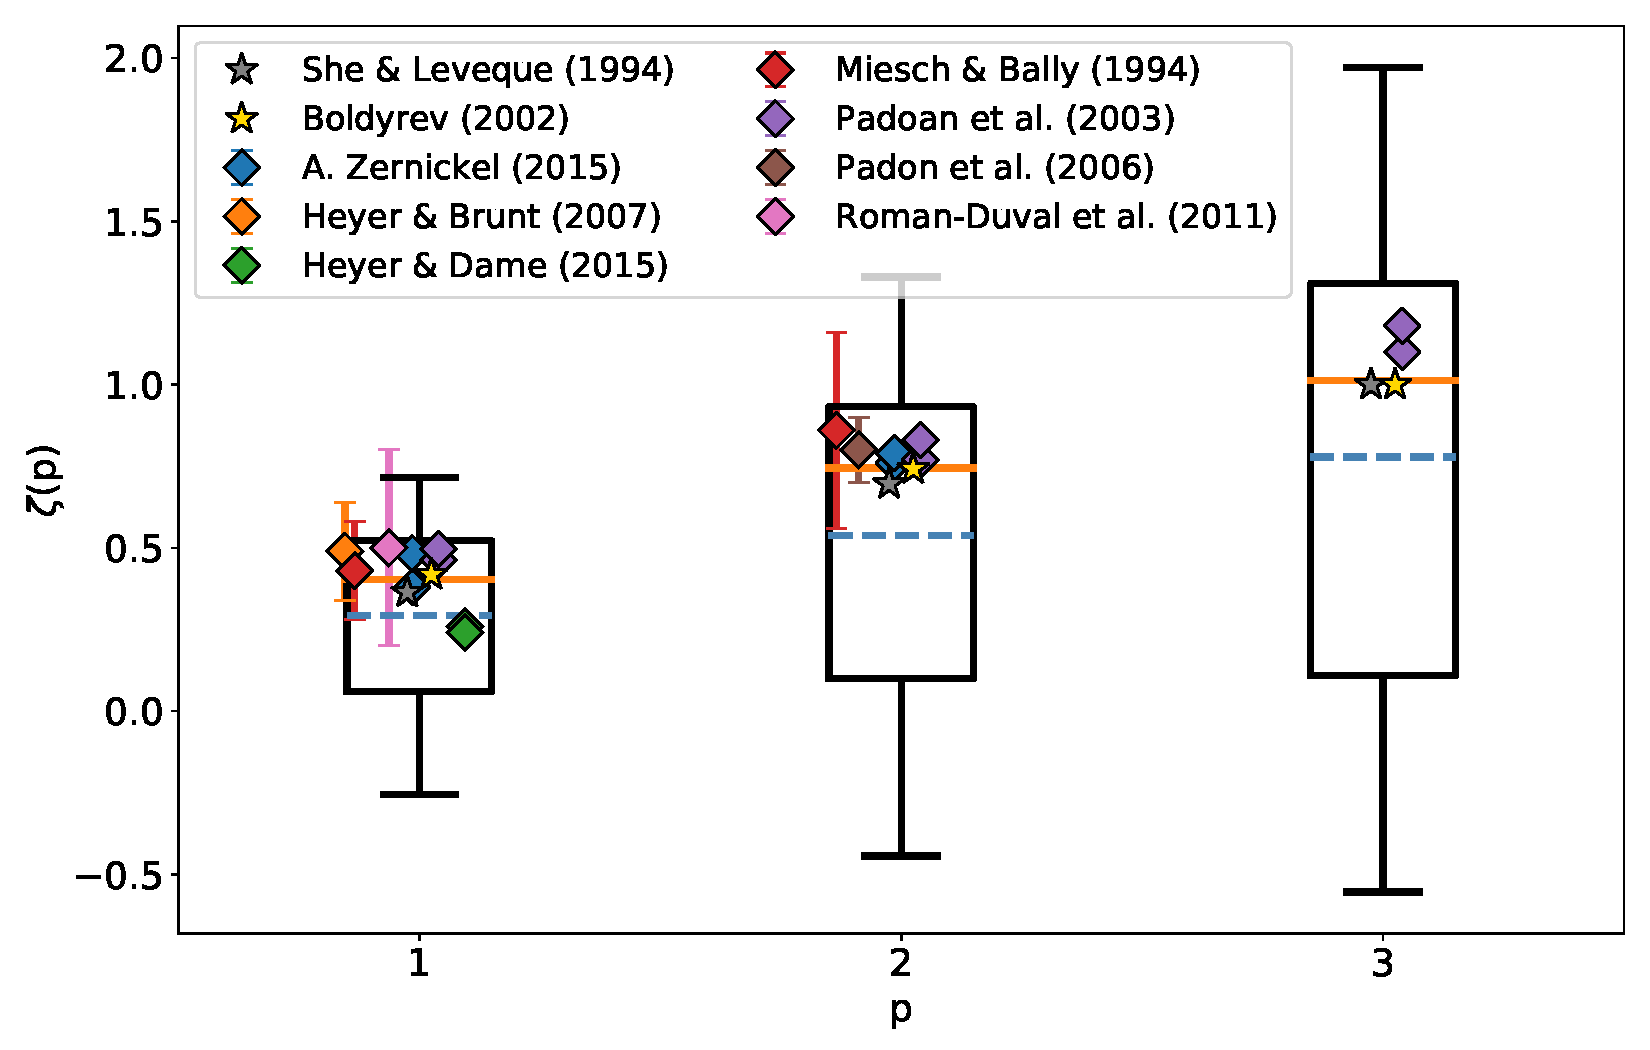
\includegraphics[width=0.49\textwidth]{compare_observations.pdf}
	\caption{Summary of measurements of $\zeta$ (\textit{abscissas}) and $Z$ (\textit{ordinates}) for orders $p=1$--3 (from \textit{left} to \textit{right}). The grey boxes represent the values presented in Sect.~\ref{results:normal}. The orange solid and blue dashed lines represent the average and median values of the distributions, respectively. The coloured star markers illustrate the predictions by \citet{She1994} and \citet{Boldyrev2002}. The coloured, circular markers summarise values found in the literature (see legend for precise references).
	}
	\label{pic:discussion:comp_observation}
\end{figure}


Compared to these measurements, the distributions of our results show a large scatter across the parameter space. 
However, we also see that there is a significant fraction of values in our models that \textbf{are consistent with the} observational findings. 
These measurements belong roughly to the evolutionary stages of the modelled clouds after having evolved for 1.5--4~Myr after the onset of self-gravity.
\citetalias{Chira2018} finds that the clouds consist of a highly hierarchical structure that is dominated by already fragmenting filaments at this point.
This means that the flows within the clouds experience a transition from cloud-scale dominated, through filament-dominated, to core-collapse driven motions; which is exactly what we observe in the VSFs, as well.
Consequently this \textbf{suggests} that the observed MCs, which show clear signs of embedded star formation activity, are in a similar stage where flows are dominated by the formation of hierarchical structures, (pre-/proto-)stellar cores or, in the case of NGC 6334, internal feedback.

We find that the interpretation of observational measurements is still difficult for several reasons:
\begin{enumerate}
\item We have already discussed in Sect.~\ref{discussion:1d} that the transformation from 3D to 1D VSFs is not trivial, in particular when the studied flows are not isotropic.
This is, for example, the case when the first structures (such as filaments or sheets) form, or the first cores collapse and accrete.
\item We have seen that interactions with SN shocks may trigger a preferred direction, that has the potential to strongly influence the measured 1D VSF.
Although the influence of shock fronts on VSFs is transient compared to the lifetime of the entire MC, it is still long enough to mimic a quasi-steady state in real observations.
Observing typical shock tracers, such as SiO, may help to identify these situations. 
\item We have neglected typical line-of-sight effects that may have a significant influence on the measurements of the local standard of rest velocity whose precision is crucial for this kind of study.
Our projections ignore optical depth effects, and reflect velocities all the way through the clouds, including high column density regions of dynamical collapse where motions are fast at small scales.  However, CO reaches optical depth of unity at relatively low column densities. This means that the observed VSFs will only reflect the motions of the surface layers of dense MCs.  
Therefore, single-tracer observations are not suitable for studying the dynamical structure of MCs. 
For a proper VSF analysis it would be advisable to use a variety of tracers to cover the different phases of the clouds, as well as to populate the statistics of lag distances more completely.
\item Only a small fraction of the listed observational studies in Table~\ref{tab:discussion:summary_obs} aimed to measure the VSFs of the respective objects directly.
In the majority of cases, the focus of the investigations was on the general budget of kinetic energy within the MC, as well as the question whether those clouds follow Larson's size-velocity relation (Eq.~[\ref{eq:larson}]).
It is unclear whether the difference between a relation of the lag distance of two particles and their relative line-of-sight velocity and the connection between the size of the entire MC and the velocity dispersion of the contained gas has always been considered.
\end{enumerate}

We recommend that both theorists and observers discuss in more detail how observational studies may use VSFs in the future.
From the theoretical point-of-view, full line radiative transfer calculations are required to better evaluate observational biases and simple projection effects.
This requires observations with a high spatial resolution of the respective MC for a wide range of lag scales and good statistics for fitting the scaling of VSF, as well as lines with well-defined line-of-sight velocities, ideally, optically thin lines of intermediate- and high-density tracers. 









\endinput
